\documentclass[preview]{standalone}

\usepackage{amsmath}
\usepackage{amssymb}
\usepackage{parskip}
\usepackage{fullpage}
\usepackage{hyperref}
\usepackage{stellar}
\usepackage{definitions}

\begin{document}

\id{functions}
\genpage

\section{Definition}

\begin{snippetdefinition}{function-definition}{Function}
    Let \(A\) and \(B\) be \set[sets].
    A \emph{function} from \(A\) to \(B\), denoted \(f\colon A\fromto B\),
    is a \binrelation \(f\) from \(A\) to \(B\) where
    \[
        \forall x \in A \exists_{=1} \, y \in B \suchthat (x,y) \in f
    \]
    The \set \(A\) is called \emph{domain} and the \set \(B\) is called \emph{codomain}. \\
    \emph{Syntax:} given a \set \(X\), \(f(X) = \{y = f(x) \suchthat x\in X\}\).
\end{snippetdefinition}

\begin{snippet}{function-diagram-illustration}
\begin{center}
    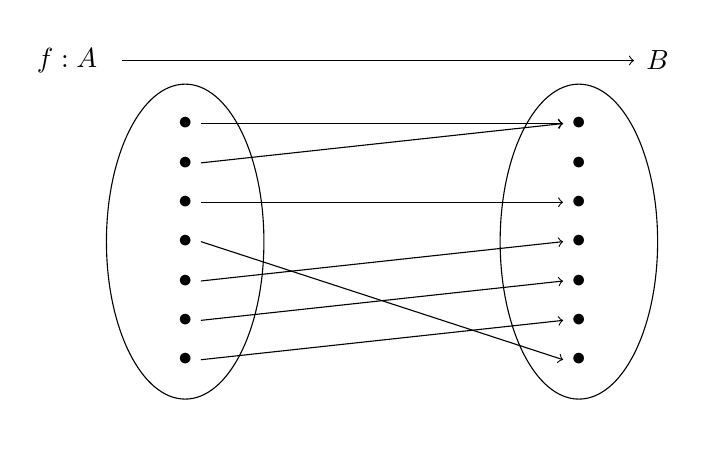
\begin{tikzpicture}
        %sets A and B
        \draw (0,0) ellipse (1 and 2);
        \draw (5,0) ellipse (1 and 2);
        \node at (-1.5,2.3) {$f:A$};
        \node at (6,2.3) {$B$};
        \draw[->] (-0.8,2.3) -- (5.7,2.3);
        
        %set A
        \node at (0,-1.5) {$\bullet$};
        \node at (0,-1) {$\bullet$};
        \node at (0,-0.5) {$\bullet$};
        \node at (0,0) {$\bullet$};
        \node at (0,0.5) {$\bullet$};
        \node at (0,1) {$\bullet$};
        \node at (0,1.5) {$\bullet$};
        
        %set B
        \node at (5,-1.5) {$\bullet$};
        \node at (5,-1) {$\bullet$};
        \node at (5,-0.5) {$\bullet$};
        \node at (5,0) {$\bullet$};
        \node at (5,0.5) {$\bullet$};
        \node at (5,1) {$\bullet$};
        \node at (5,1.5) {$\bullet$};
        
        %arrows
        \draw[->] (0.2,-1.5) -- (4.8,-1);
        \draw[->] (0.2,-1) -- (4.8,-0.5);
        \draw[->] (0.2,-0.5) -- (4.8,0);
        \draw[->] (0.2,0) -- (4.8,-1.5);
        \draw[->] (0.2,0.5) -- (4.8,0.5);
        \draw[->] (0.2,1) -- (4.8,1.5);
        \draw[->] (0.2,1.5) -- (4.8,1.5);
    
        %spacer
        \node at (0,2.6) {\phantom{}};
        \node at (0,-2.2) {\phantom{}};
    \end{tikzpicture}
\end{center}
\end{snippet}

\plain{Every function has an arrow for each element in the domain.}

\begin{snippetdefinition}{function-image-definition}{Image}
    Let \(f\colon X\fromto Y\) be a \function.
    The \emph{image} of \(f\) is defined as
    \[ \text{Im}(f) = \{y \in Y \suchthat y=f(x), x \in X \} \]
\end{snippetdefinition}

\section{Properties}

\begin{snippetdefinition}{injectivity-definition}{Injectivity}
    A \function \(f \colon A\fromto B\) is \emph{injective} if
    \[
        \forall a,b \in A, f(a) = f(b) \implies a = b
    \]
\end{snippetdefinition}

\begin{snippetdefinition}{surjectivity-definition}{Surjectivity}
    A \function \(f \colon A\fromto B\) is \emph{surjective} if
    \[
        \forall b \in B \exists a \suchthat f(a)=b
    \]
\end{snippetdefinition}

\begin{snippetdefinition}{bijectivity-definition}{Bijectivity}
    A \function \(f \colon A\fromto B\) is \emph{bijective} if
    it has a one-to-one correspondence between each element of \(A\) and  \(B\).
\end{snippetdefinition}

\begin{snippetcorollary}{bijectivity-equiv-inj-and-surj}{Bijectivity properties}
    A \function \(f \colon A\fromto B\) is bijective \ifandonlyif it is both \injective and \surjective.
\end{snippetcorollary}

\begin{snippetdefinition}{function-composition-definition}{Function composition}
    Let \(\Phi \colon A \fromto B\) and \(\Psi \colon B \fromto C\) be \function[functions].
    The \emph{composition} of \(\Phi\) and \(\Psi\) is given by
    \[
        (\Phi \circ \Psi)(x) \triangleq \Psi(\Phi(x))
    \]
\end{snippetdefinition}

\subsection{Invertibility}

\begin{snippetdefinition}{identity-function-definition}{Identity function}
    Let \(X\) be a \set. Then, the \emph{identity function} on \(X\)
    is the \function
    \[
        \text{Id}_X \colon X \fromto X
    \]
    such that \(\text{Id}_X(x) \triangleq x\).
\end{snippetdefinition}

\begin{snippetdefinition}{inverse-function-definition}{Inverse function}
    Let \(A\) and \(B\) be sets. A \function \(f\colon A \fromto B\) is \emph{invertible}
    if there exists another function \(f^{-1}\colon B \fromto A\), called the \emph{inverse function},
    such that
    \begin{itemize}
        \item \(\forall x \in A, f^{-1}(f(x)) = \identity_A\);
        \item \(\forall y \in B, f(f^{-1}(y)) = \identity_B\).
    \end{itemize}
\end{snippetdefinition}

\subsection{Periodic functions}

\begin{snippetdefinition}{periodic-function-definition}{Periodic Function}
    A \function \(f\) is periodic with a period \(T\) if
    \[
        f(x) = f(x + kT), \quad k \in \naturalnumbers
    \]
\end{snippetdefinition}

\begin{snippetdefinition}{odd-function-definition}{Odd Function}
    A \function \(f\) is \emph{odd} if
    \[
        f(-x) = -f(x)
    \]
\end{snippetdefinition}

\begin{snippetdefinition}{even-function-definition}{Even Function}
    A \function \(f\) is even if
    \[
        f(-x) = f(x)
    \]
\end{snippetdefinition}

\begin{snippetdefinition}{equaliser-definition}{Equaliser}
    Let \(X,Y\) be \set[sets] and \(f,g \colon X \fromto Y\) be \function[functions].
    Then, the \emph{equalizer} of \(f\) and \(g\) is
    \[
        \text{Eq}(f,g) \triangleq
        \{
            x\in X \suchthat f(x) = g(x)
        \}
    \]
\end{snippetdefinition}

\end{document}